\documentclass[11pt,spanish]{article}
\usepackage[T1]{fontenc}
\usepackage{selinput}
\usepackage{amsmath, amsthm, amsfonts, mathtools}
\usepackage{babel}
\usepackage{clrscode}
\usepackage[margin=1.2in]{geometry}
\usepackage[usenames,dvipsnames]{xcolor}
\usepackage{listings}
\usepackage{array}
\usepackage{tikz}
\usetikzlibrary{
  shapes.multipart,
  matrix,
  positioning,
  shapes.callouts,
  shapes.arrows,
  calc,
  automata,
  arrows,
  topaths}


\let\oldepsilon\epsilon
\renewcommand{\epsilon}{\varepsilon}

\SelectInputMappings{%
  aacute={á},
  ntilde={ñ},
  Euro={€}
}
 
\definecolor{codegreen}{rgb}{0,0.6,0}
\definecolor{codegray}{rgb}{0.5,0.5,0.5}
\definecolor{codepurple}{rgb}{0.58,0,0.82}
\definecolor{backcolour}{rgb}{0.95,0.95,0.92}
\definecolor{mypink1}{rgb}{0.858, 0.188, 0.478}
\definecolor{mypink2}{RGB}{222, 148, 148}
\definecolor{pastelpink}{rgb}{1.0, 0.82, 0.86}
\definecolor{myyellow}{RGB}{245,177,0}
\definecolor{mysalmon}{RGB}{255,145,73}

\newcommand{\tab}[1]{\hspace{.05\textwidth}\rlap{#1}}
\newcommand{\itab}[1]{\hspace{0em}\rlap{#1}}
 
\lstdefinestyle{mystyle}{
    backgroundcolor=\color{white},   
    commentstyle=\color{codegreen},
    keywordstyle=\color{blue},
    numberstyle=\tiny\color{codegray},
    stringstyle=\color{codepurple},
    basicstyle=\footnotesize,
    breakatwhitespace=false,         
    breaklines=true,                 
    captionpos=b,                    
    keepspaces=true,                 
    numbers=left,                    
    numbersep=5pt,                  
    showspaces=false,                
    showstringspaces=false,
    showtabs=false,                  
    tabsize=2
}
 
\lstset{style=mystyle}
 
\title{Descripción de solución Problema A \\
Sección: 01 \\}
\author{Sebastián Valencia Calderón 201111578 \\
  Laura Ávila Bermudez 201212736 \\
  Grupo 08
}

\begin{document}
\maketitle

\begin{enumerate}
	\item \textbf{Algoritmo de solución}. El algoritmo de solución, se divide en dos partes, el cómputo del cuadrado de área máxima dentro de la entrada, y el cómputo del rectángulo de área máxima dentro del mismo. Para el primero, se usó programación dinámica, el algoritmo, usa espacio adicional para llevar cuanta de los lados máximos encontrados hasta ahora. Por ejemplo, si se considera el arreglo rectángular de bits mostrado, el espacio necesario, con su configuración, semuestra a constinuación, además, la explicación de cada item de la nueva matriz: 
	
	\[
\begin{bmatrix}
    0 & 1 & 1 & 0 & 0 & 1 & 0 \\
    1 & 0 & 1 & 0 & 1 & 1 & 1 \\
    1 & 1 & 0 & 0 & 1 & 1 & 0
\end{bmatrix}
\Rightarrow
\begin{bmatrix}
	0 & 0 & 0 & 0 & 0 & 0 & 0 & 0 \\
    0 & 0 & 1 & 1 & 0 & 0 & 1 & 0 \\
    0 & 1 & 0 & 1 & 0 & 1 & 1 & 1 \\
    0 & 1 & 1 & 0 & 0 & 1 & 2 & 0
\end{bmatrix}
\]

En ésta nueva matriz, los bordes superior e izquierdo, así como su intersección, tienen el valor de $0$. Mientras tanto, la submatriz restante, tiene un cero $0$ si en ésa misma posición ajustada, la matriz original lo tiene, de lo contrario (la posición ajustada de la matriz original es un uno), el elemento de ésa posición, se obtiene a partir de la fórmula:

$$\min \left( A_{i - 1, j}, A_{i - 1, j - 1}, A_{i, j - 1}\right) + 1$$

En la fórmula, $A$ es la nueva matriz. La entrada máxima de ésta, corresponde al lado del cuadrado más grande dentro de la matriz original. La igualdad de cada elemento de la matriz se muestra a continuación ($M$ es la matriz original):

\[
 A_{i, j} =
  \begin{cases}
   0 & \text{if } i = 0 \vee j = 0 \vee B_{i - 1, j - 1} = 0  \\
   \min \left( A_{i - 1, j}, A_{i - 1, j - 1}, A_{i, j - 1}\right) + 1       & \text{otherwise }
  \end{cases}
\]

Para hallar el rectángulo, se cuentan los unos arriba de cada fila de la matriz, si es un uno, sino, se deja cero, a partir de éste arreglo, se halla el rectángulo más grande dentro de éste histograma. Asimismo, se acumula el máximo. Es decir, para cada fila de la matriz original, se genera un arreglo que cuente para cada posición de la fila, los unos por encima de ésta entrada en caso de que la misma sea un uno. De lo contrario, se coloca cero. éste nuevo arreglo, se pasa para calcular el rectángulo de área máxima dentro de éste histograma.


\item \textbf{Análisis temporal y espacial de la solución}. El tamaño del problema, es la tupla $M, N$. La complejidad espacial de la solución ingenua, es $O(1)$. La complejidad  temporal, se deduce de manera análitica, contando el número de ejecución de cada inStrucción. Para ésto, se cuenta con la siguiente expresión, donde como operaciones de costo $\Theta(1)$, se consideraron, la suma, la resta, la multiplicación, la división, obtener la longitud de un arreglo, indexar un arreglo, asignar, y comparar átomos de lenguaje.
	
	$$T_{t}(M, N) = \sum_{i=0}^{M} \left( \sum_{j=0}^{N} \left[ \Theta(1) + \sum_{p1=0}^{i + 1} \sum_{p2=p1}^{i+1} \sum_{q1=0}^{j+1} \sum_{q2=q1}^{j+1} \left[ \Theta(1) + \sum_{r=p1}^{p2+1} \Theta(1) + \Theta(1) \right]  + \Theta(1)\right] \right)$$
	
	$$T_{t}(M, N) = \sum_{i=0}^{M}{\sum_{j=0}^{N}{\left(\left(\sum_{{\it p_1}=0}^{i+1}{
 \sum_{{\it p_2}={\it p_1}}^{i+1}{\left({\it p_2}-{\it p_1}+4\right)}
 }\right)\,\sum_{{\it q_1}=0}^{j+1}{\left(-{\it q_1}+j+2\right)}+2
 \right)}}$$
 
 $$T_{t}(M, N) = {{M^4\,N^3+2\,M^3\,N^3+M^2\,N^3}\over{144}}+{{2\,M^3\,N^3+3\,M^2\,N
 ^3+M\,N^3}\over{12}}+ \dots$$
 
 $$T_{t}(M, N) = O(M^4\,N^3)$$
 
 Para la solución propuesta, se tiene, la expresión:
 
 $$T_{t}(M, N) = 2 \sum_{i=0}^{M} \left[ \sum_{j=0}^{N} \Theta(1)\right]+ \Theta(1) + 2 \sum_{i=0}^{N} \Theta(1) + \Theta(1)$$
 
 $$T_{t}(M, N) = 2\,\left(M+1\right)\,\left(N+1\right)+2\,\left(N+1\right)+2 = O(MN)$$
 
 Para una comprabación empírica de ésto, se generó un conjunto de entradas aleatorias para todos los tamaños (small, medium, big). El programa de generación, se muestra a continuación:
 
 \lstinputlisting[language=Python]{../src/measure.py}
 
 A partir de las entradas generadas, se corren los programas y se mide su tiempo según la metodología de Bob Sedgewick. A continuación, se grafican los tiempos, si se asume que la entrada es el producto $MN$, ésto para evitar usar gráficas en tercera dimensión. En la gráfica, la linea roja es el tiempo de la solución ingenua, mientras la azul, la solución planteada.Además, puede verse que la solución planteada, es $M^4N^2/MN = M^3N^2$ veces mejor que la ingenua.
 
 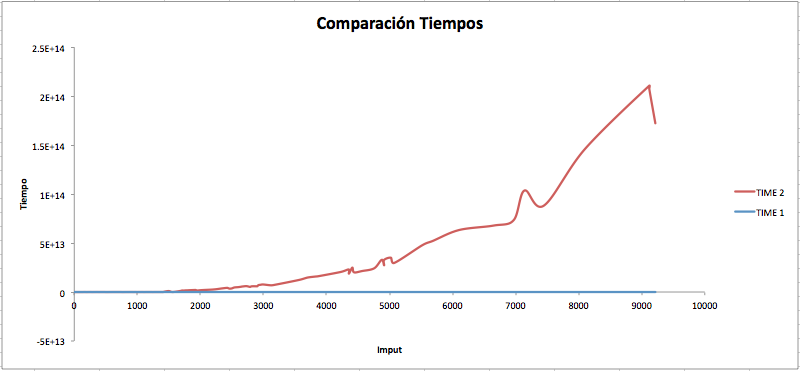
\includegraphics[scale=0.5]{compare.png}
 
 \item \textbf{Comentarios finales} En la solución se observa un desempeño dependiente linealmente del producto de las dimensiones de las entradas. Además, se percibe una simplificación muy severa en el uso de la notación $O$, pues la complejidad de la solución ingenua, desprecia varios términos del resultado de la sumatoria. Si $M = N$, la solucion ingenua es $O(M^7)$, mientras la propuesta es $O(M^2)$, ambas soluciones perteneces a la clase P de complejidad. Sin embargo, al hacer la prueba sobre 100 datos de cada tipo de entrada, se percibe que la solución propuesta no demora casi nada, mientras la otra, demora mucho más de una hora y media. 
 
 
	
		

  
\end{enumerate}
\iffalse
\lstinputlisting[language=Pascal]{src/maxSubarray.pas}
\fi

% Bibliografía.
%-----------------------------------------------------------------

\end{document}